\documentclass[11pt]{article}

\usepackage[T1]{fontenc}
\usepackage[utf8]{inputenc}
\usepackage{lmodern}
\usepackage[margin=1in]{geometry}
\usepackage{graphicx}
\usepackage{booktabs}
\usepackage{tabularx}
\usepackage{multirow}
\usepackage{array}
\usepackage{amsmath,amssymb}
\usepackage{xcolor}
\usepackage{tikz}
\usetikzlibrary{arrows.meta,positioning,fit,calc}
\usepackage{caption}
\usepackage{placeins}
\usepackage{url}
\usepackage[numbers,sort&compress]{natbib}
\usepackage[hidelinks]{hyperref}
\usepackage{microtype}

\graphicspath{{figures/}}

% Keep floats near their first citation in dense Method/Results.
\renewcommand{\topfraction}{0.85}
\renewcommand{\bottomfraction}{0.8}
\renewcommand{\textfraction}{0.1}
\renewcommand{\floatpagefraction}{0.7}
\setcounter{topnumber}{4}
\setcounter{bottomnumber}{2}
\setcounter{totalnumber}{6}

\hypersetup{
  pdftitle={Optimizing Consecutive Tool Calling for Small Language Models on Edge Devices},
  pdfauthor={Sanskar Thapa}
}

\newcommand{\todo}[1]{\textcolor{red!65!black}{\textbf{TODO:} #1}}
\newcommand{\pp}{\,pp}

\title{Optimizing Consecutive Tool Calling for\\ Small Language Models on Edge Devices}
\author{Sanskar Thapa\\[0.4em]
{\normalsize Master's thesis draft (due December 2026)}\\[0.2em]
{\normalsize \url{https://github.com/sskarz/Thesis}}}
\date{September 2026}

\begin{document}
\maketitle

\begin{abstract}
Small language models (SLMs) with fewer than five billion parameters are attractive for on-device agents, but consecutive, stateful tool calling remains unreliable. This paper evaluates quantized SLMs on the Berkeley Function Calling Leaderboard (BFCL) v4, taking multi-turn \emph{execution} accuracy on the 200-case \texttt{multi\_turn\_base} split as the primary agentic metric and single-turn abstract-syntax-tree (AST) accuracy as a supporting diagnostic. All own measurements use llama.cpp on a MacBook Pro with Apple M4~Pro and Metal; NVIDIA Jetson replication is left open.

On single-turn AST (990 cases; parallel categories excluded after a serving-layer grammar bug), Qwen3.5-4B Q4\_K\_M reaches 817/990 (82.53\%), ahead of Qwen2.5-3B (76.06\%), FunctionGemma-270M (39.90\%), and Llama-3.2-3B (36.87\%). Schema-aware type coercion plus a system prompt lifts Llama's \texttt{multiple} accuracy from 41.5\% to 92.0\%: much of that gap was argument serialization, not tool selection.

On multi-turn, Gemma-4-E2B-it Q4\_K\_M scores 54/200 (27.0\%) with native function calling and 61/200 (30.5\%) with Instruction-Followed Function Calling (IFFC; JSON tool calls in ordinary assistant text). Inference-time working memory, a gated stop-on-repeat guardrail, and a one-pass OODA-style status card raise accuracy to 34.0\%, 32.5\%, and 35.5\%. Best-of-N majority voting ($N{=}5$) on IFFC plus working memory reaches 73/200 (36.5\%) at roughly $7\times$ generate cost. Constrained decoding (10.5\%) and a live tool-name automaton (13.5\%) are scored regressions. Supervised fine-tuning on IFFC mixes collapses to 0.5\% when empty-list stop targets dominate, recovers to 15.0\% after curriculum repair, and still underperforms the untuned base model. Direct Preference Optimization has passed a 10-example health gate; full-train BFCL results are pending.
\end{abstract}

\section{Introduction}
\label{sec:intro}

An on-device agent must do more than emit a single well-formed API call. It has to choose a tool, fill typed arguments, incorporate execution feedback, and decide when \emph{not} to call anything. Errors cascade: a wrong function, a stringified integer, or a hallucinated call can leave the environment in a state that later turns cannot recover. Cloud-scale models are routinely scored for these behaviors. Edge and local-first deployments instead need models that fit in a few gigabytes and return interactive latency on consumer silicon.

This work studies SLMs under five billion parameters served with llama.cpp~\cite{llamacpp} on Apple Silicon. The motivating setting is a local agent loop: the model proposes calls, a harness executes them against a live backend, and the next user turn depends on the resulting state. Two failure families dominate that loop. \emph{Format} failures are syntactic or channel mismatches---native \texttt{tool\_calls} versus JSON in text, stringly-typed arguments, truncated parallel grammars---that can look like reasoning errors on a leaderboard. \emph{State} failures are agentic: the model calls something valid but drifts from the environment, repeats a completed action, or stops too early.

The questions are empirical:

\begin{enumerate}
  \item How accurately do quantized SLMs perform single-turn tool selection and multi-turn consecutive calling on BFCL v4 when served locally with Metal?
  \item How much of measured failure is format and serving infrastructure versus genuine multi-turn state tracking?
  \item Which inference-time interventions (output channel, working memory, decoding constraints, test-time voting, simple guardrails) and which training-time interventions (supervised fine-tuning, preference optimization) move the primary multi-turn metric?
\end{enumerate}

\paragraph{Contributions.}
At claim level, rather than as a list of harness flags:

\begin{enumerate}
  \item \textbf{A local BFCL v4 baseline} for four quantized SLMs on single-turn AST, plus Gemma-4-E2B-it on multi-turn execution, all on MacBook Pro M4~Pro / llama.cpp Metal. No own NVIDIA RTX~4090 numbers are reported.
  \item \textbf{Format is first-order.} Switching Gemma from native tool calls to IFFC JSON-in-text gains ${+}3.5$\pp\ on \texttt{multi\_turn\_base}. Llama type coercion plus a system prompt lifts \texttt{multiple} from 41.5\% to 92.0\%. A published xLAM-1b checkpoint scores 0\% on this native-tools harness and only 3\% on a format-matched channel---neither figure is the public overall BFCL number.
  \item \textbf{Light inference interventions move consecutive accuracy on the base Gemma checkpoint}, up to 36.5\% with expensive majority vote and 35.5\% with a cheap OODA-style card. Constrained decoding and a live name automaton do not help.
  \item \textbf{Standard IFFC supervised fine-tuning is brittle on this mix.} Empty-list stop-after-tools targets collapse the model to 0.5\%; mix surgery recovers 15.0\% but does not beat untuned IFFC (30.5\%) or native calling (27.0\%). Working memory that helps the base model does not help that checkpoint.
  \item \textbf{Preference optimization is the open training path.} A Direct Preference Optimization (DPO) smoke run passed a 10-example health gate. A capped full train is in flight; this draft reports no $N{=}200$ DPO accuracy.
\end{enumerate}

Section~\ref{sec:related} defines BFCL and the methods we compare. Section~\ref{sec:method} describes each intervention once. Section~\ref{sec:setup} states the experimental setup. Sections~\ref{sec:results-st}--\ref{sec:results-train} report results by what helped, what did not, and what is still open. Section~\ref{sec:discussion} discusses format versus reasoning and cost. Section~\ref{sec:roadmap} is the roadmap. Appendix~\ref{app:runs} maps method names to evaluation-log run IDs.

\section{Background and Related Work}
\label{sec:related}

\subsection{BFCL and consecutive tool calling}
The Berkeley Function Calling Leaderboard (BFCL) and the Gorilla line of work evaluate language models as API callers~\cite{patil2023gorilla,patil2024bfcl}. We use BFCL v4.

Single-turn categories are scored with an AST checker: the model sees a user query and a tool schema and must emit a call (or none) whose structure matches a reference, allowing equivalent argument order. Categories include \texttt{simple} (one available function), \texttt{multiple} (several functions, pick the right one), \texttt{parallel} / \texttt{parallel\_multiple} (several calls in one turn), \texttt{irrelevance} (the query needs no call), and Java / JavaScript typed variants.

Multi-turn categories are scored with an \emph{execution} checker. The model enters an agent loop; tools run against a live backend; instance state is compared to a reference trajectory. The four slices are \texttt{multi\_turn\_base} (full tool set), \texttt{miss\_func} (some tools withheld until later), \texttt{miss\_param} (required arguments omitted from the query), and \texttt{long\_context} (large histories). This paper's optimization target is \texttt{multi\_turn\_base} ($N{=}200$). Paper percentages on that slice are \emph{not} public overall-BFCL leaderboard scores, which mix many categories and often different serving stacks.

\subsection{Native versus instruction-followed function calling}
\paragraph{Native function calling (NFC).}
The server is given OpenAI-style \texttt{tools} and the model is expected to return structured \texttt{tool\_calls}. llama.cpp may compile a grammar (GBNF) once chat-template trigger tokens appear. This is the default production channel for many local stacks.

\paragraph{Instruction-followed function calling (IFFC).}
Taheri et al.~\cite{taheri2026iffc} argue that small models can follow JSON instructions more reliably than native tool APIs. Their paper reports large gains on BFCL v3 \emph{single-turn} suites, often with a dual-model design that separates a QA model from a small reasoning model (their Algorithm~1). We implement only Appendix~B: the \emph{same} model emits a JSON list of \texttt{\{function\_name, parameters\}} objects in assistant text, with no native \texttt{tools} field. Dual-model IFFC is deferred (Section~\ref{sec:roadmap}).

\subsection{Structured decoding, templates, and test-time compute}
XGrammar-2 describes efficient dynamic structured generation, including TagDispatch for tag-triggered grammar switches~\cite{dong2026xgrammar2}. That work reports, for example, lifting Llama-3.2-3B correct-call rates from 33\% to 78\% \emph{under its engine}---prior-work figures, not our measurements. Our constrained-decoding ablation approximates TagDispatch with two stock llama-server requests and is not full XGrammar-2. Guided generation more broadly is studied by Willard and Louf~\cite{willard2023outlines}; format restrictions can also hurt quality~\cite{tam2024format}.

He et al.~\cite{he2025gst} propose seven-step guided-structured templates (GST) that improve function calling on BFCL v2. We overlay their Detail template as a prompt on NFC; the checker executes native \texttt{tool\_calls} and ignores GST draft text. This is not a grammar and not IFFC.

Snell et al.~\cite{snell2024testtime} frame test-time compute versus parameter scaling. Our Best-of-N is majority vote over sampled tool-call tuples, not tree search and not a learned verifier.

\subsection{Working memory and specialist SLM callers}
ACON compresses older turns with LLM summarization~\cite{xu2025acon}. Our STATE overlay is a harness-written key-value snapshot from \emph{executed} tool results, not an LLM summary.

Error taxonomies for sub-7B callers often rank type mismatch among dominant failures~\cite{liu2024apigen}. Specialist models such as FunctionGemma~\cite{google2025functiongemma}, Hammer~\cite{ye2025hammer}, and xLAM~\cite{zhang2024xlam} show that fine-tuning and format design can make small models competitive. We treat type coercion as an inference-time mitigation that does not change weights, and we score a published xLAM-1b GGUF on \emph{this} harness rather than citing the public overall figure (${\sim}78.94\%$) as a reproduction.

\subsection{Training-time methods}
QLoRA is the standard efficient-finetuning reference~\cite{dettmers2023qlora}; we train LoRA adapters with MLX on Apple Silicon~\cite{mlx}, not QLoRA-on-CUDA. ToolACE~\cite{liu2024toolace} and xLAM supply the IFFC JSON-in-text mix. Direct Preference Optimization~\cite{rafailov2023dpo} and dialogue-level variants such as DiaTool-DPO~\cite{jung2025diatool} motivate a preference path after SFT proved brittle; our DPO evidence in this draft is a health gate, not a BFCL score.

\section{Method}
\label{sec:method}

Figure~\ref{fig:channels} summarizes the interventions. Every multi-turn method is scored with the same BFCL execution checker; only the request shape, decoding constraints, prompt overlay, working-memory injection, sampling, or weights change. Method caveats that are easy to over-claim are collected in Appendix~\ref{app:caveats}.

\begin{figure}[!htbp]
\centering
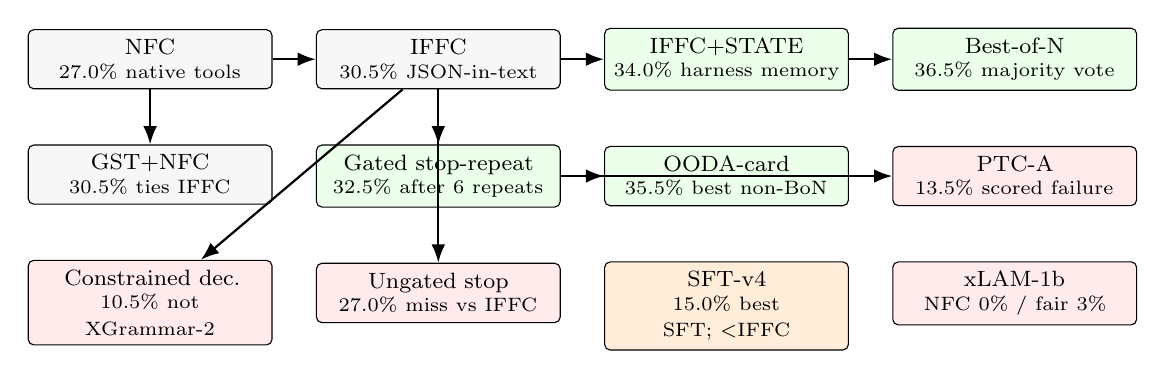
\begin{tikzpicture}[
  font=\footnotesize,
  box/.style={draw, rounded corners=2pt, align=center, inner sep=3.5pt, fill=gray!6, text width=2.85cm},
  neg/.style={draw, rounded corners=2pt, align=center, inner sep=3.5pt, fill=red!8, text width=2.85cm},
  win/.style={draw, rounded corners=2pt, align=center, inner sep=3.5pt, fill=green!8, text width=2.85cm},
  recov/.style={draw, rounded corners=2pt, align=center, inner sep=3.5pt, fill=orange!15, text width=2.85cm},
  arr/.style={-{Latex}, thick}
]
\node[box] (nfc) {NFC\\[-1pt]{\scriptsize 27.0\% native tools}};
\node[box, right=0.55cm of nfc] (iffc) {IFFC\\[-1pt]{\scriptsize 30.5\% JSON-in-text}};
\node[win, right=0.55cm of iffc] (state) {IFFC$+$STATE\\[-1pt]{\scriptsize 34.0\% harness memory}};
\node[win, right=0.55cm of state] (bon) {Best-of-N\\[-1pt]{\scriptsize 36.5\% majority vote}};

\node[box, below=0.7cm of nfc] (gst) {GST$+$NFC\\[-1pt]{\scriptsize 30.5\% ties IFFC}};
\node[win, below=0.7cm of iffc] (stop) {Gated stop-repeat\\[-1pt]{\scriptsize 32.5\% after 6 repeats}};
\node[win, below=0.7cm of state] (ooda) {OODA-card\\[-1pt]{\scriptsize 35.5\% best non-BoN}};
\node[neg, below=0.7cm of bon] (ptc) {PTC-A\\[-1pt]{\scriptsize 13.5\% scored failure}};

\node[neg, below=0.7cm of gst] (cd) {Constrained dec.\\[-1pt]{\scriptsize 10.5\% not XGrammar-2}};
\node[neg, below=0.7cm of stop] (ungated) {Ungated stop\\[-1pt]{\scriptsize 27.0\% miss vs IFFC}};
\node[recov, below=0.7cm of ooda] (sft) {SFT-v4\\[-1pt]{\scriptsize 15.0\% best SFT; $<$IFFC}};
\node[neg, below=0.7cm of ptc] (xlam) {xLAM-1b\\[-1pt]{\scriptsize NFC 0\% / fair 3\%}};

\draw[arr] (nfc) -- (iffc);
\draw[arr] (iffc) -- (state);
\draw[arr] (state) -- (bon);
\draw[arr] (nfc) -- (gst);
\draw[arr] (iffc) -- (stop);
\draw[arr] (stop) -- (ooda);
\draw[arr] (iffc) -- (ungated);
\draw[arr] (iffc) -- (cd);
\draw[arr] (stop) -- (ptc);
\end{tikzpicture}
\caption{Interventions on BFCL v4 \texttt{multi\_turn\_base} ($n{=}200$), Gemma-4-E2B-it Q4\_K\_M unless noted, MacBook Pro M4~Pro / llama.cpp Metal. Green: methods that beat plain IFFC (30.5\%) on the \emph{base} checkpoint. Orange: best supervised recovery, still below IFFC. Red: scored misses or closed failures. xLAM is an external published checkpoint on the same slice, not a Gemma training method. SFT v1/v2 collapse (0.5\%) is omitted for space; see Table~\ref{tab:scoreboard}.}
\label{fig:channels}
\end{figure}

\FloatBarrier

\subsection{Output channels}
\label{sec:method-channels}

\paragraph{NFC.}
The harness sends \texttt{tools} and \texttt{tool\_choice=auto}. Assistant outputs are native \texttt{tool\_calls}. This is the Gemma multi-turn baseline and the channel used for the xLAM native-tools probe.

\paragraph{IFFC.}
Following Appendix~B of~\cite{taheri2026iffc}, we omit \texttt{tools}. The system prompt asks for a JSON list of \texttt{function\_name} / \texttt{parameters} objects in assistant text. Tool results return as user-role messages. Trajectories are mapped to the same BFCL function strings used by NFC.

\paragraph{xLAM JSON channel.}
Salesforce xLAM-1b-fc-r is trained to emit \texttt{\{"tool\_calls":[\ldots]\}} in content, not OpenAI \texttt{tool\_calls}. A format adapter parses that JSON and executes tools. This is a channel fix for a published checkpoint, not a new training method.

\paragraph{Shell dialect.}
An allowlisted Unix-like text dialect is mapped onto GorillaFileSystem calls (e.g., \texttt{cd notes} $\to$ \texttt{cd(folder='notes')}) and scored only on the 13 filesystem-only IDs in \texttt{multi\_turn\_base}. It is a format ablation, not a substitute for the 200-entry score.

\subsection{Inference overlays on IFFC or NFC}
\label{sec:method-overlays}

\paragraph{Guided-structured templates (GST$+$NFC).}
The He et al.\ Detail curriculum is prepended as a one-shot system prompt on top of NFC~\cite{he2025gst}. The model is asked to write a \texttt{[GST]} scaffold before native \texttt{tool\_calls}. The checker ignores the scaffold.

\paragraph{Harness STATE.}
IFFC is unchanged as a channel. After each successful tool execution, the harness writes a compact \texttt{[STATE]} snapshot from real results and attaches it in user messages. The last two turns stay verbatim; older raw dumps are dropped. This is not LLM summarization.

\paragraph{Best-of-N (BoN).}
On the IFFC$+$STATE channel, each agent step samples $N{=}5$ completions at temperature 0.7, majority-votes the \texttt{(function\_name, arguments)} tuple, executes the winner once, and continues. Latency is roughly $N$ greedy decodes. This is not a verifier.

\paragraph{Stop-on-repeat.}
After a tool observation, if the proposed call set is a subset of already-executed calls (or consecutive identical sets), the harness stops the turn without re-executing. An \emph{ungated} version fires immediately; a \emph{tightened} version waits until six assistant tool-turns of the same observation (\texttt{MIN}${}=6$) before treating observe-same as a stop, while consecutive identical calls still stop immediately. This is a decode/harness guardrail, not a retrain.

\paragraph{OODA-card.}
A one-pass status card with fields for goal, filled slots, last observation, and a suggested next action is stacked on tightened stop-repeat. The ``next'' field is advisory. This is not a four-stage OODA controller and not the STATE overlay.

\paragraph{TagDispatch-style constrained decoding (CD).}
Stock llama-server does not expose intra-request tag-triggered grammar switches. We approximate TagDispatch with two requests and never send \texttt{tools}, so native tools GBNF does not activate. Pass~1 constrains the completion to an empty list or a list of live \texttt{function\_name} values. Pass~2 constrains arguments for the selected names via \texttt{json\_schema}. This is not full XGrammar-2 (no intra-request tag switch, two HTTP requests per tool invocation).

\paragraph{Prefix-tree name constraint (PTC-A).}
A live deterministic finite automaton constrains the tool \emph{name} while arguments remain free. This is inspired by prefix-tree constrained decoding; it is not a reproduction of that literature's F1 numbers, and it is not the two-pass CD ablation above.

\subsection{Type coercion}
\label{sec:method-coerce}

Llama-3.2-3B often selects the correct function on \texttt{multiple} but serializes integers, floats, arrays, and objects as JSON strings. We apply (i)~a system prompt requiring native JSON types and (ii)~schema-aware post-hoc coercion of argument values to the BFCL parameter types. Both are inference-time only.

\subsection{Parallel grammar bug}
\label{sec:method-parallel}

When \texttt{tools} are present, llama-server may compile a tools grammar whose repetition structure mismatches the model's trained multi-call delimiters. Generation can stop after the first closing tag, truncating parallel output. A bypass (\texttt{tool\_choice none} with content parsing) is implemented; re-measurement is pending, so tables still report 0\% for \texttt{parallel} and \texttt{parallel\_multiple}.

\subsection{Supervised fine-tuning and preference optimization}
\label{sec:method-sft}

We train LoRA adapters on Gemma-4-E2B-it with mlx-lm~\cite{mlx} using an IFFC JSON-in-text mix (ToolACE multi-turn~\cite{liu2024toolace} plus stratified xLAM~\cite{zhang2024xlam}), fuse a best-validation checkpoint, quantize to Q4\_K\_M, and evaluate under IFFC on \texttt{multi\_turn\_base}. Mix variants drop empty-list assistant targets after tool results, drop first-turn empty answers, and try turn-0 / state-consistency filters. A serve-time diagnostic strips trailing assistant \texttt{[]} from chat history without retraining; we do not treat that diagnostic as a method.

A 100-update DPO smoke ($\beta{=}0.2$) from the untouched Gemma MLX base is used only as a health gate (call volume, parseability, first-turn tool use on 10 IDs). A capped full DPO train is in flight. This paper does not report a DPO \texttt{multi\_turn\_base} accuracy.

\section{Experimental Setup}
\label{sec:setup}

\subsection{Hardware and serving}
All own experiments run on a MacBook Pro with Apple M4~Pro (48~GB), Metal GPU acceleration, llama.cpp build 8111 (commit \texttt{11c325c6e}), compiled with \texttt{-DGGML\_METAL=ON}. Models are served with \texttt{llama-server --jinja}, flash attention on, and full GPU offload (\texttt{-ngl 99}). This draft does not claim RTX~4090 results. NVIDIA Jetson Orin Nano Super (CUDA, 8~GB) replication is open (Section~\ref{sec:roadmap}).

\subsection{Models}
Single-turn matrix (Q4\_K\_M unless noted): Qwen2.5-3B-Instruct, Llama-3.2-3B-Instruct, Qwen3.5-4B, and FunctionGemma-270M-IT (bf16; the published precision). Multi-turn primary model: Gemma-4-E2B-it Q4\_K\_M. External baseline: Salesforce xLAM-1b-fc-r Q4\_K\_M. Decoding for reported accuracy uses temperature 0.0 except BoN (temperature 0.7, $N{=}5$). Overnight multi-turn jobs use \texttt{-np 4 -c 65536}.

\subsection{Evaluation protocol}
Single-turn: BFCL AST checker. Multi-turn: BFCL execution checker. FunctionGemma control-token outputs are normalized with a dedicated parser when llama-server does not already map them to \texttt{tool\_calls}. Weighted single-turn averages exclude \texttt{parallel} and \texttt{parallel\_multiple} (990 remaining cases). Failure buckets use one primary error per failed entry unless noted as raw eval-error rows. Chronological run IDs from the evaluation log are demoted to Appendix~\ref{app:runs}; the main text uses method names.

\section{Single-turn Results}
\label{sec:results-st}

Table~\ref{tab:single-turn} and Figure~\ref{fig:accuracy} report per-category AST accuracy. Qwen2.5-3B leads \texttt{simple} and \texttt{multiple}. Qwen3.5-4B leads the non-parallel weighted average via strong irrelevance detection (91.25\%). Llama-3.2-3B is weak on core Python calling and near floor on irrelevance, but strongest on Java (54/100) and JavaScript (35/50). FunctionGemma, at 270M parameters, exceeds Llama on \texttt{multiple} (59.00\% versus 33.50\%).

\begin{table}[htbp]
\centering
\caption{Single-turn BFCL v4 AST accuracy on MacBook Pro M4~Pro / llama.cpp Metal. Parallel categories are 0\% pending re-run after a llama-server tools GBNF truncation bug (Section~\ref{sec:method-parallel}) and are excluded from the weighted average.}
\label{tab:single-turn}
\footnotesize
\setlength{\tabcolsep}{4pt}
\begin{tabular}{@{}lrrrr@{}}
\toprule
Category ($n$) & Qwen2.5-3B & Llama-3.2-3B & Qwen3.5-4B & FuncGemma-270M \\
 & Q4\_K\_M & Q4\_K\_M & Q4\_K\_M & bf16 \\
\midrule
Simple (400) & 373/400 (93.25\%) & 207/400 (51.75\%) & 361/400 (90.25\%) & 205/400 (51.25\%) \\
Multiple (200) & 185/200 (92.50\%) & 67/200 (33.50\%) & 181/200 (90.50\%) & 118/200 (59.00\%) \\
Parallel (200)$^*$ & 0/200 (0.00\%) & 0/200 (0.00\%) & 0/200 (0.00\%) & 0/200 (0.00\%) \\
Par.\ multiple (200)$^*$ & 0/200 (0.00\%) & 0/200 (0.00\%) & 0/200 (0.00\%) & 0/200 (0.00\%) \\
Irrelevance (240) & 141/240 (58.75\%) & 2/240 (0.83\%) & 219/240 (91.25\%) & 48/240 (20.00\%) \\
Java (100) & 37/100 (37.00\%) & 54/100 (54.00\%) & 39/100 (39.00\%) & 15/100 (15.00\%) \\
JavaScript (50) & 17/50 (34.00\%) & 35/50 (70.00\%) & 17/50 (34.00\%) & 9/50 (18.00\%) \\
\midrule
Weighted, excl.\ parallel$^*$ & 753/990 (76.06\%) & 365/990 (36.87\%) & \textbf{817/990 (82.53\%)} & 395/990 (39.90\%) \\
\bottomrule
\end{tabular}\\[0.4em]
{\raggedright\scriptsize $^*$Parallel / parallel\_multiple: 0\% attributed to llama-server tools GBNF truncation; bypass implemented; re-run not yet scored. Gemma-4-E2B-it is multi-turn only and is not in this table.\par}
\end{table}

\begin{figure}[!htbp]
\centering
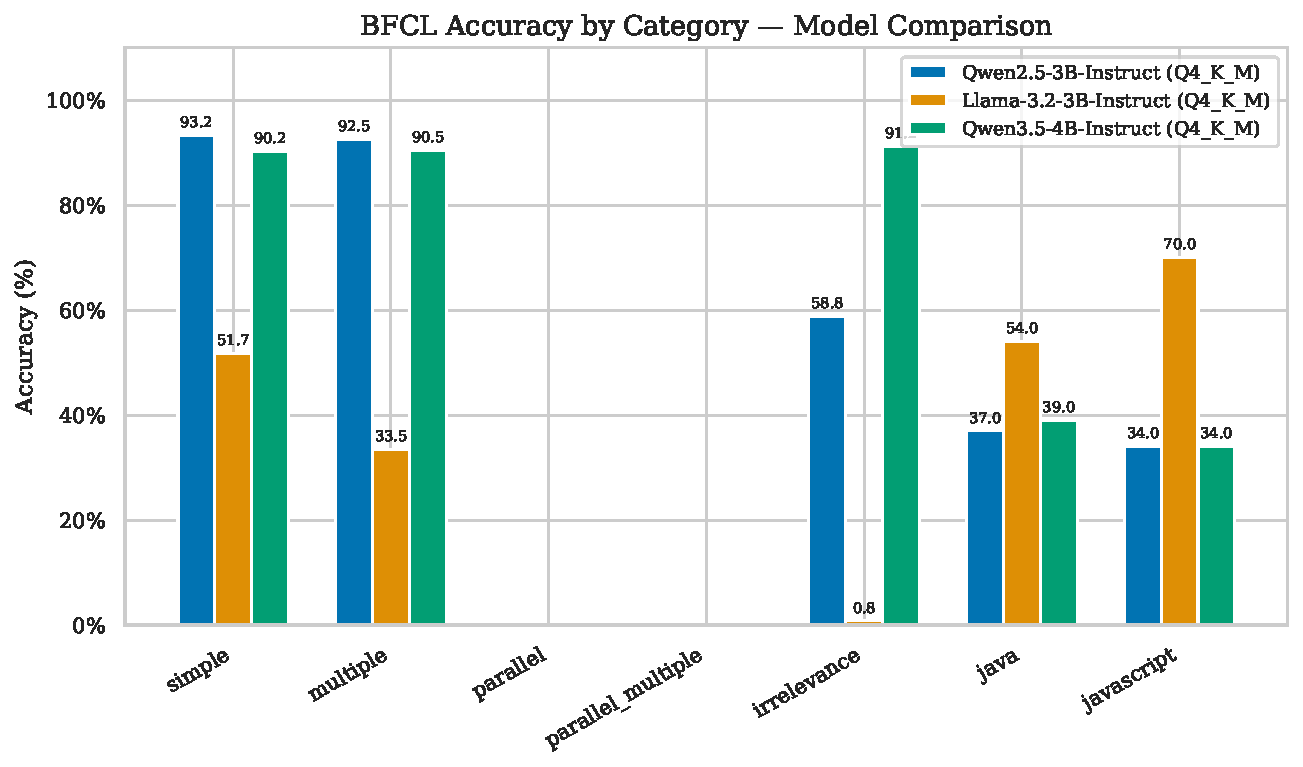
\includegraphics[width=0.92\textwidth]{accuracy_comparison.pdf}
\caption{Single-turn BFCL v4 AST accuracy by category for Qwen2.5-3B, Llama-3.2-3B, Qwen3.5-4B, and FunctionGemma-270M. MacBook Pro M4~Pro, llama.cpp Metal. Parallel bars are the invalidated 0\% scores (GBNF truncation), not a claimed model limitation.}
\label{fig:accuracy}
\end{figure}

\subsection{Type coercion recovers Llama's multiple gap}
\label{sec:results-coerce}

On the full \texttt{multiple} category, combining a system prompt and schema-aware type coercion raises Llama-3.2-3B from 41.5\% to 92.0\% (Table~\ref{tab:coerce}). Coercion alone accounts for most of the lift; Qwen models barely move because they already emit native JSON types. Apparent inter-family gaps on AST can therefore be formatting rather than tool selection. The 41.5\% diagnostic baseline is a separate snapshot from the 33.50\% (67/200) Llama \texttt{multiple} cell in Table~\ref{tab:single-turn}; both are measured, not reconciled by invention.

\begin{table}[htbp]
\centering
\caption{Inference-time type-coercion diagnostic on BFCL v4 \texttt{multiple} ($n{=}200$). MacBook Pro M4~Pro / llama.cpp Metal. No weight updates.}
\label{tab:coerce}
\small
\begin{tabular}{@{}lrrr@{}}
\toprule
Method & Llama-3.2-3B & Qwen2.5-3B & Qwen3.5-4B \\
\midrule
Baseline & 41.5\% & 93.0\% & 94.5\% \\
System prompt only & 57.0\% (${+}15.5$\pp) & 94.5\% (${+}1.5$\pp) & 94.5\% ($\pm 0$) \\
Type coercion only & 87.5\% (${+}46.0$\pp) & 93.0\% ($\pm 0$) & 94.5\% ($\pm 0$) \\
Prompt $+$ coercion & \textbf{92.0\% (${+}50.5$\pp)} & 94.5\% (${+}1.5$\pp) & 94.5\% ($\pm 0$) \\
\bottomrule
\end{tabular}
\end{table}

\FloatBarrier

\section{Multi-turn Results: Inference-Time Interventions}
\label{sec:results-mt}

Unless noted, scores are Gemma-4-E2B-it Q4\_K\_M on BFCL v4 \texttt{multi\_turn\_base} ($n{=}200$), Mac Metal. Table~\ref{tab:scoreboard} is the primary scoreboard. Figure~\ref{fig:scoreboard} shows an earlier Gemma-only chart (through SFT-v6); later rows live in the table. NFC secondary slices, scored only for the native baseline, are much harder: \texttt{miss\_func} 16/200 (8.0\%), \texttt{miss\_param} 39/200 (19.5\%), \texttt{long\_context} 22/200 (11.0\%).

\begin{figure}[!htbp]
\centering
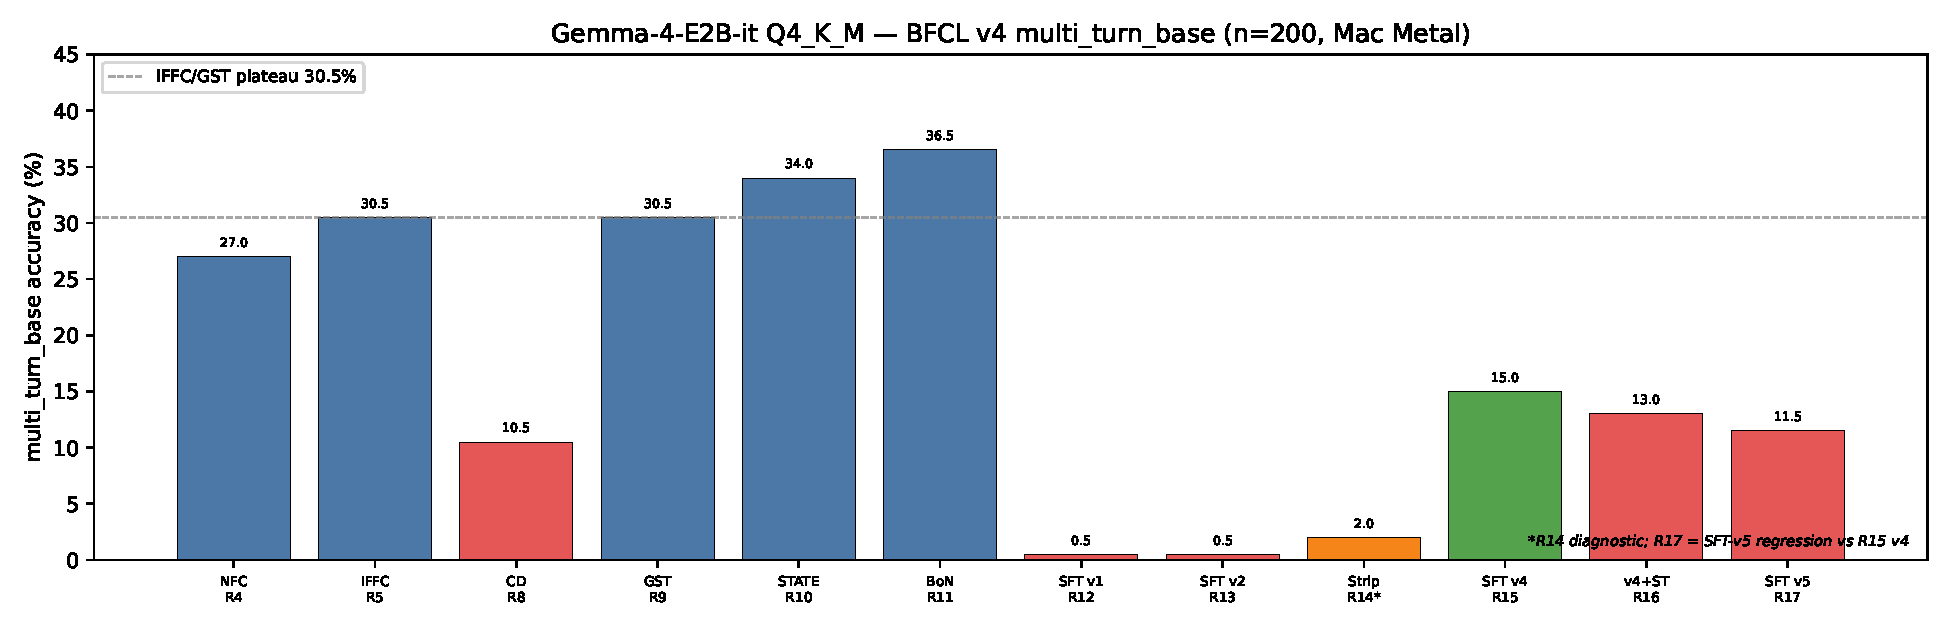
\includegraphics[width=0.98\textwidth]{multiturn_scoreboard.pdf}
\caption{Gemma-4-E2B-it Q4\_K\_M execution accuracy on \texttt{multi\_turn\_base} for the early intervention set (native calling through SFT-v6). Hardware: MacBook Pro M4~Pro, llama.cpp Metal. Later conditions---stop-on-repeat, OODA-card, PTC-A, and xLAM---are in Table~\ref{tab:scoreboard}, which is the complete scoreboard. Constrained decoding is a TagDispatch-style two-pass approximation, not full XGrammar-2.}
\label{fig:scoreboard}
\end{figure}

\begin{table}[htbp]
\centering
\caption{Primary multi-turn scoreboard: BFCL v4 \texttt{multi\_turn\_base} ($n{=}200$), MacBook Pro M4~Pro / llama.cpp Metal. Gemma-4-E2B-it Q4\_K\_M except xLAM-1b-fc-r Q4\_K\_M. $\Delta$ is versus plain IFFC (61/200). Paper percentages on this slice are not public overall-BFCL scores.}
\label{tab:scoreboard}
\footnotesize
\setlength{\tabcolsep}{3.5pt}
\begin{tabular}{@{}p{4.6cm}rrl@{}}
\toprule
Condition & Score & Acc. & vs IFFC / note \\
\midrule
Best-of-N $N{=}5$ on IFFC$+$STATE & 73/200 & \textbf{36.5\%} & ${+}6.0$\pp; ${\sim}7\times$ wall; majority vote \\
OODA-card (on gated stop-repeat) & 71/200 & 35.5\% & ${+}5.0$\pp; best non-BoN \\
IFFC$+$STATE (harness memory) & 68/200 & 34.0\% & ${+}3.5$\pp \\
Gated stop-repeat (\texttt{MIN}${}=6$) & 65/200 & 32.5\% & ${+}2.0$\pp; harness guardrail \\
IFFC (JSON-in-text) & 61/200 & 30.5\% & baseline channel \\
GST$+$NFC (He Detail prompt) & 61/200 & 30.5\% & tie via 19-row swap, not a win \\
NFC (native \texttt{tool\_calls}) & 54/200 & 27.0\% & ${-}3.5$\pp \\
Ungated stop-repeat & 54/200 & 27.0\% & ${-}3.5$\pp; same level as NFC, different method \\
SFT-v4 IFFC (best SFT recovery) & 30/200 & 15.0\% & ${-}15.5$\pp; still below NFC \\
PTC-A (live name DFA) & 27/200 & 13.5\% & ${-}17.0$\pp; scored failure \\
SFT-v6 IFFC & 26/200 & 13.0\% & miss vs SFT-v4 \\
SFT-v4 $+$ STATE & 26/200 & 13.0\% & STATE helps base, not this ckpt \\
SFT-v5 IFFC & 23/200 & 11.5\% & regression vs SFT-v4 \\
Constrained decoding (not XGrammar-2) & 21/200 & 10.5\% & ${-}20.0$\pp \\
xLAM-1b JSON channel & 6/200 & 3.0\% & fair channel; still very low \\
SFT-v2 $+$ strip trailing \texttt{[]} & 4/200 & 2.0\% & diagnostic, not a method \\
SFT-v1 / SFT-v2 IFFC & 1/200 & 0.5\% & empty-\texttt{[]} collapse \\
xLAM-1b NFC & 0/200 & 0.0\% & format-channel collapse \\
\bottomrule
\end{tabular}
\end{table}

\FloatBarrier

\subsection{What helped}
\label{sec:results-helped}

\paragraph{IFFC over NFC (${+}3.5$\pp).}
JSON-in-text scores 61/200 versus 54/200 native. Pairwise, both fail on 124 entries; IFFC rescues 22 and regresses 15. Empty-turn error rows fall roughly 118$\to$41 and state-mismatch rows 136$\to$60. Once calls parse, residual error is environment fidelity, not the channel label.

\paragraph{Harness STATE (${+}3.5$\pp over IFFC).}
Working memory from executed tools scores 68/200 (34.0\%), the first method above the 30.5\% IFFC/GST plateau on \emph{base} Gemma. Versus IFFC the overlap is shared 48, rescue 20, regress 13 (net ${+}7$). Empty turns fall 41$\to$31 while state mismatch does not improve (60$\to$64). STATE appears to help forgotten calls more than env-diff fidelity. Stored response blobs contain literal \texttt{[STATE]} in 0/200 rows, as expected: STATE is conversation context written by the harness.

\paragraph{Gated stop-on-repeat (${+}2.0$\pp over IFFC).}
Waiting until six observe-same tool-turns before forcing a stop scores 65/200 (32.5\%). Stop flags fall from 37/200 (ungated) to 3/200, all still failures. VehicleControlAPI state-mismatch counts return to the IFFC baseline (22, versus 33 ungated). This is a harness guardrail on the base checkpoint, not a training win, and it remains below STATE (34.0\%) and BoN (36.5\%).

\paragraph{OODA-card (${+}3.0$\pp over gated stop-repeat).}
The one-pass status card scores 71/200 (35.5\%): best non-BoN accuracy, still 1.0\pp\ below BoN. State-mismatch errors remain high (71 of 129 failures). Latency is compatible with the gated-stop run (median TTFT 517.8~ms versus 630.5~ms). The card helps consecutive accuracy without fixing state tracking.

\paragraph{Best-of-N majority vote (${+}2.5$\pp over STATE, ${\sim}7\times$ cost).}
Sampling $N{=}5$ on IFFC$+$STATE scores 73/200 (36.5\%), the best measured inference result. Versus greedy STATE: shared 56, BoN-only 17, greedy-only 12. Table~\ref{tab:bon-cost} reports the cost. On an edge Mac this is a deliberate test-time trade, not a default serving mode.

\begin{table}[htbp]
\centering
\caption{Cost of BoN $N{=}5$ versus greedy IFFC$+$STATE on Gemma-4-E2B-it Q4\_K\_M, \texttt{multi\_turn\_base} $n{=}200$, Mac M4~Pro Metal, \texttt{-np 4 -c 65536}. From multi-turn timings. No per-request throughput row was stored for BoN; we do not invent tok/s.}
\label{tab:bon-cost}
\small
\begin{tabular}{@{}lrrr@{}}
\toprule
Metric & IFFC$+$STATE & BoN $N{=}5$ & Ratio \\
\midrule
Avg.\ predicted time / entry & ${\sim}150$~s & ${\sim}1318$~s & ${\sim}8.8\times$ \\
Avg.\ prompt time / entry & ${\sim}22$~s & ${\sim}210$~s & ${\sim}9.5\times$ \\
Avg.\ API calls & 8.4 & 42.7 & ${\sim}5.1\times$ \\
Avg.\ turns & ${\sim}3.67$ & ${\sim}3.67$ & ${\sim}1\times$ \\
Generate wall & ${\sim}3.0$~h & ${\sim}21.3$~h & ${\sim}7\times$ \\
\midrule
Accuracy & 68/200 (34.0\%) & 73/200 (36.5\%) & ${+}2.5$\pp \\
\bottomrule
\end{tabular}
\end{table}

\paragraph{Llama type coercion.}
Covered in Section~\ref{sec:results-coerce}: a large single-turn \texttt{multiple} lift from formatting, not from better tool choice.

\subsection{What did not help}
\label{sec:results-hurt}

\paragraph{Ungated stop-on-repeat (27.0\%, ${-}3.5$\pp versus IFFC).}
Stopping at the first repeated observation matches NFC's 54/200 but is a different method, not a reproduction of native calling. All 37 stop flags land among the 146 failures (zero stopped-and-correct). VehicleControlAPI state mismatches rise 22$\to$33. Early stopping helps only loop-dominated traces; on healthy base Gemma it cuts good trajectories.

\paragraph{GST$+$NFC ties IFFC, does not beat it.}
61/200 via a 19-row swap each way (both correct 42). Versus NFC: ${+}3.5$\pp. Empty turns fall to 31 (NFC 59, IFFC 41) while state mismatch rises to 79 (NFC 68, IFFC 60). The checklist increases calling volume, not environment-state tracking.

\paragraph{Constrained decoding (10.5\%).}
The two-pass name-then-args approximation scores 21/200: ${-}16.5$\pp versus NFC and ${-}20.0$\pp versus IFFC (179 errors). Syntactic validity is not consecutive correctness on this stack. This is not a claim about full XGrammar-2 TagDispatch.

\paragraph{PTC-A (13.5\%, closed).}
A live tool-name automaton scores 27/200: ${-}22.0$\pp versus OODA-card, ${-}19.0$\pp versus gated stop-repeat, ${-}17.0$\pp versus IFFC. State mismatch rises to 102. We treat this line as a scored failure and do not remix it as the next accuracy bet. A related PTC-B variant remains unrun by design.

\paragraph{xLAM on this harness (0\% then 3\%).}
Under NFC, the published xLAM-1b-fc-r Q4\_K\_M GGUF scores 0/200: every error is an empty turn-0 tool-call list. The server generated tokens (mean 3.63 recorded API-layer calls), but NFC never parses assistant \texttt{content}. The JSON-in-text adapter scores 6/200 (3.0\%): tools actually run (mean 50.47 API calls) and then over-call, fail to parse (111/200 unparseable flags), and drift (128 state mismatches). Neither 0\% nor 3\% is the published overall BFCL figure of ${\sim}78.94\%$, which is a different mixture of categories and serving. Same-slice contrast: Gemma NFC is 27.0\%.

\paragraph{Shell-as-action (filesystem-only, $n{=}13$).}
On the 13 GorillaFileSystem-only IDs, NFC scores 3/13 (23.1\%), IFFC 1/13 (7.7\%), shell v1 1/13, shell v2 0/13 (Table~\ref{tab:shell}). Mapping polish does not beat native calling on this slice. These percentages are not comparable to the 200-entry scoreboard; the ablation is closed.

\begin{table}[htbp]
\centering
\caption{Shell-as-action format ablation on GorillaFileSystem-only \texttt{multi\_turn\_base} IDs ($n{=}13$), Gemma-4-E2B-it Q4\_K\_M, Mac Metal. Not comparable to the 200-entry scoreboard.}
\label{tab:shell}
\small
\begin{tabular}{@{}lrrl@{}}
\toprule
Mode & Score & Acc. & Pass IDs \\
\midrule
NFC & 3/13 & 23.1\% & \texttt{\_3}, \texttt{\_12}, \texttt{\_29} \\
IFFC & 1/13 & 7.7\% & \texttt{\_12} \\
Shell v1 & 1/13 & 7.7\% & \texttt{\_12} \\
Shell v2 & 0/13 & 0.0\% & --- \\
\bottomrule
\end{tabular}
\end{table}

\FloatBarrier

\section{Multi-turn Results: Training-Time Interventions}
\label{sec:results-train}

\subsection{SFT empty-list mixes collapse}
\label{sec:results-sft-collapse}

LoRA on the original IFFC mix scores 1/200 (0.5\%). A live single-step probe still emits valid IFFC JSON, so this is not a parser or chat-template failure. The dominant behavior is early stop with an empty list \texttt{[]} after tool results. The MLX mix contains 5520 assistant \texttt{[]} targets, all from ToolACE (32.5\% of ToolACE assistant turns; xLAM 0\%). After a ``Function execution results'' user message, 78.1\% of assistant targets are \texttt{[]} (2121 empty versus 596 continue). That teaches stop-after-tools; BFCL multi-turn requires continued calls on later user turns.

Filtering 334 mid-trajectory empty-after-exec rows while keeping 552 terminal empty-after-exec examples (SFT-v2) again scores 1/200. Empty primary fails rise 101$\to$167. Figure~\ref{fig:sft} shows the scored slice. Stripping trailing assistant \texttt{[]} from chat history at serve time, without retraining, reaches only 4/200 (2.0\%). Turn-0 empty errors remain 153. History bookkeeping does not rescue a never-start collapse.

\begin{figure}[!htbp]
\centering
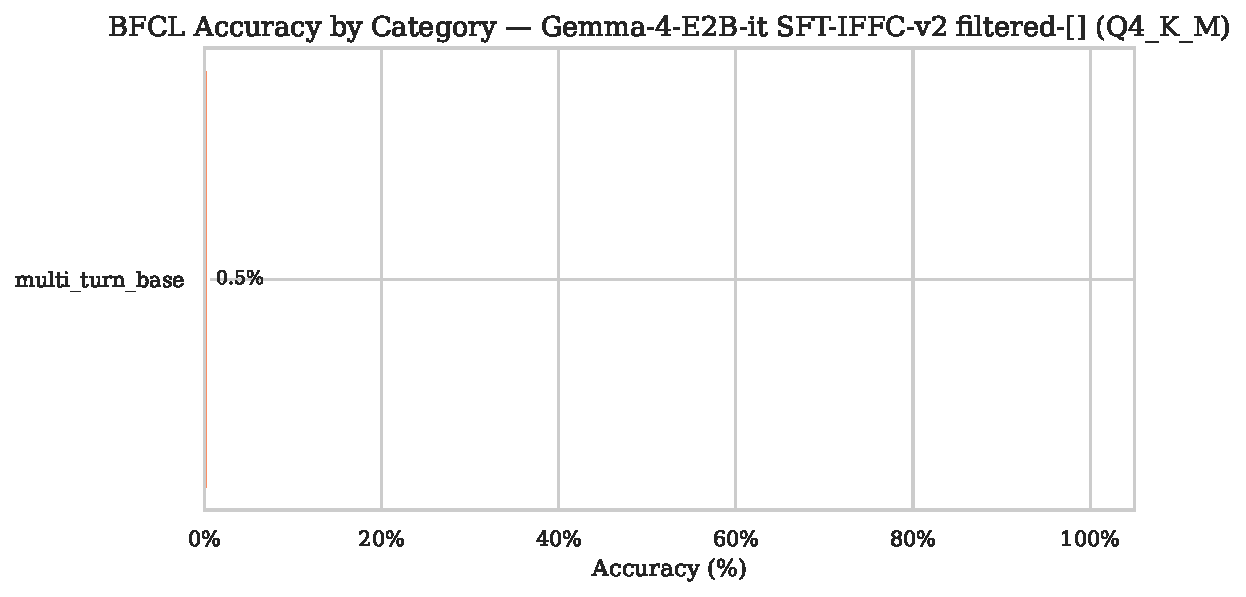
\includegraphics[width=0.82\textwidth]{sft_v2_accuracy.pdf}
\caption{SFT-IFFC-v2 accuracy on the scored BFCL v4 slice. Gemma-4-E2B-it fused Q4\_K\_M, MacBook Pro M4~Pro / llama.cpp Metal, IFFC channel. Score 1/200 (0.5\%) --- a scored negative; dropping non-terminal empty lists did not recover.}
\label{fig:sft}
\end{figure}

\subsection{SFT-v4 recovers empty lists, not consecutive accuracy}
\label{sec:results-sft-v4}

Dropping empty-after-exec targets (including terminal), adding recovery rows, and dropping first-assistant-empty and clarifying empty-after-user \texttt{[]} yields 30/200 (15.0\%): ${+}29$ entries versus SFT-v2, still ${-}31$ versus IFFC and ${-}24$ versus NFC. Correct-set overlap versus IFFC: shared 23, SFT-only 7, IFFC-only 38. Empty-turn primaries fall 167$\to$2. Residual error is state mismatch (109) and under-call (59), including 35 turn-0 under-calls. This is the best SFT recovery in the study. It is not a win over the untuned base model.

\subsection{Further mix surgery regresses; STATE does not transfer}
\label{sec:results-sft-later}

IFFC$+$STATE on the same v4 GGUF scores 26/200 (13.0\%): ${-}2.0$\pp versus plain IFFC on that checkpoint. Contrast: STATE on base Gemma was ${+}3.5$\pp. Empty stays rare (3); residual remains state mismatch (112) and under-call (59).

SFT-v5 keeps the v4 empty-recovery curriculum and adds turn-0 completeness plus state-consistency filters (${\sim}29850$ train rows). It scores 23/200 (11.5\%): a regression versus v4. Empty primaries fall to 0/177, but state mismatch rises to 133. Mean API calls jump to 40.27 (v4 was 17.32).

SFT-v6 keeps v4 empty/recovery plus only the state-inconsistency drop (turn-0 underspecification filters off). It scores 26/200 (13.0\%): a miss versus v4, a modest lift versus v5. Empty remains essentially suppressed (1). Mean API calls return to 13.34. State mismatch is 118 and under-call 55.

Thin filter ablations on this ToolACE$+$xLAM IFFC family are exhausted for now. A later quota-remix smoke (SFT v9.2, 10 IDs) failed a health gate (mean 25.7 API calls, 6/10 traces hit the step limit) and is parked; that gate is not a BFCL percentage.

\subsection{DPO: health gate passed, full-train results pending}
\label{sec:results-dpo}

A 100-update DPO smoke ($\beta{=}0.2$, LoRA, fused Q4\_K\_M) passed the same style of 10-ID health gate used to reject collapsed SFT smokes: mean API calls 4.4 (band 4--8.3), 0/10 step-limit hits, 0/10 unparseable IFFC, 7/10 first-turn tool uses. That is evidence the training stack did not immediately collapse. It is not a \texttt{multi\_turn\_base} score.

A capped full DPO train is in flight. This draft reports no $N{=}200$ DPO accuracy, does not treat the smoke checkpoint as a scoreboard row, and does not claim a method win. Preference-pair auditing (advance versus loop) remains open (Section~\ref{sec:roadmap}).

\FloatBarrier

\section{Failure Modes and Serving Cost}
\label{sec:results-fail}

\subsection{Residual errors are state mismatch and under-call}
Figure~\ref{fig:fail} and Tables~\ref{tab:fail}--\ref{tab:fail-later} use one primary error per failed entry. After IFFC, residual errors are state mismatch and under-call, not parse failure. BoN cuts state mismatch (64$\to$53) while empty turns rise slightly (31$\to$36). SFT v1/v2 collapse into empty-turn dominance. SFT-v4 largely fixes empty turns and shifts the residual onto state mismatch and under-call; later SFT mixes keep empty rare and worsen or fail to beat that state residual. Gated stop-repeat returns state-mismatch counts to the IFFC baseline; OODA-card still leaves 71 state mismatches; PTC-A inflates them to 102.

On IFFC$+$STATE, 64 state-mismatch entries concentrate in VehicleControl (22) and GorillaFileSystem (21). BoN keeps VehicleControl at 22 and cuts filesystem mismatches to 13. Those two backends remain the practical bottleneck for consecutive correctness.

\begin{figure}[!htbp]
\centering
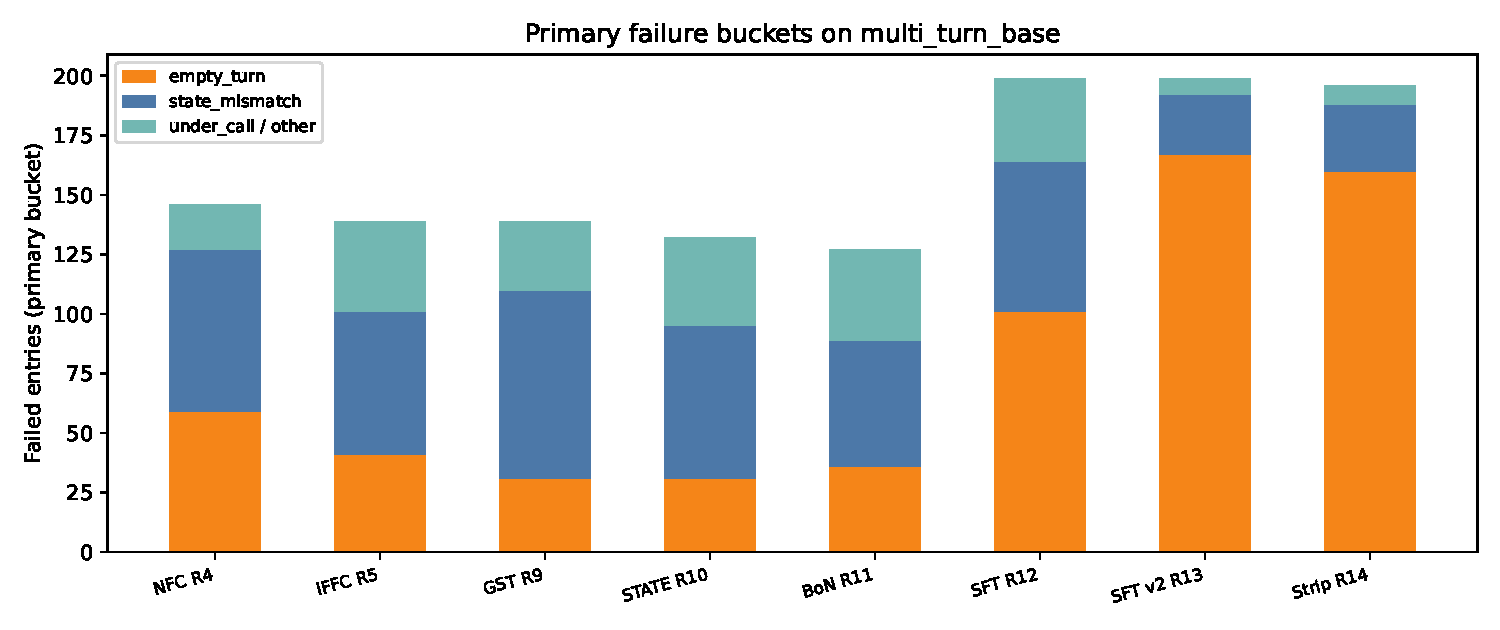
\includegraphics[width=0.98\textwidth]{failure_buckets.pdf}
\caption{Primary failure-bucket stack for Gemma-4-E2B-it Q4\_K\_M on \texttt{multi\_turn\_base} ($n{=}200$), Mac M4~Pro / llama.cpp Metal, covering native calling through SFT-v6. One primary label per failed entry. Stop-on-repeat, OODA-card, and PTC-A are in Table~\ref{tab:fail-later}.}
\label{fig:fail}
\end{figure}

\begin{table}[htbp]
\centering
\caption{Primary failure buckets (one error per failed entry) on Gemma-4-E2B-it Q4\_K\_M, \texttt{multi\_turn\_base}. Failed entries: NFC 146, IFFC 139, CD 179, GST 139, STATE 132, BoN 127, SFT-v1 199, SFT-v2 199, strip-\texttt{[]} 196, SFT-v4 170, v4$+$STATE 174, SFT-v5 177, SFT-v6 174.}
\label{tab:fail}
\footnotesize
\setlength{\tabcolsep}{1.8pt}
\begin{tabular}{@{}lrrrrrrrrrrrrr@{}}
\toprule
Bucket & NFC & IFFC & CD & GST & STATE & BoN & v1 & v2 & strip & v4 & v4S & v5 & v6 \\
\midrule
Empty turn & 59 & 41 & 14 & 31 & 31 & 36 & 101 & 167 & 160 & 2 & 3 & 0 & 1 \\
Under-call / miss.\ GT & 19 & 38 & 70 & 29 & 37 & 38 & 35 & 7 & 8 & 59 & 59 & 44 & 55 \\
State mismatch & 68 & 60 & 95 & 79 & 64 & 53 & 63 & 25 & 28 & 109 & 112 & 133 & 118 \\
\midrule
Failed entries & 146 & 139 & 179 & 139 & 132 & 127 & 199 & 199 & 196 & 170 & 174 & 177 & 174 \\
\bottomrule
\end{tabular}
\end{table}

\begin{table}[htbp]
\centering
\caption{Primary failure buckets for later harness interventions on the same Gemma checkpoint and slice. Counts sum to failed entries (200 minus correct).}
\label{tab:fail-later}
\small
\begin{tabular}{@{}lrrrr@{}}
\toprule
Bucket & Ungated stop & Gated stop & OODA-card & PTC-A \\
\midrule
Empty turn & 40 & 38 & 17 & 17 \\
Under-call / miss.\ GT & 31 & 37 & 41 & 54 \\
State mismatch & 75 & 60 & 71 & 102 \\
\midrule
Failed entries & 146 & 135 & 129 & 173 \\
Accuracy & 27.0\% & 32.5\% & 35.5\% & 13.5\% \\
\bottomrule
\end{tabular}
\end{table}

\subsection{Serving performance on M4~Pro}
Figures~\ref{fig:perf}--\ref{fig:mem} and Table~\ref{tab:perf} report dedicated metrics (3 warmup $+$ 50 controlled requests). FunctionGemma is the latency and throughput winner; Qwen3.5-4B trades speed for the best non-parallel weighted AST accuracy among the four single-turn models.

\begin{figure}[!htbp]
\centering
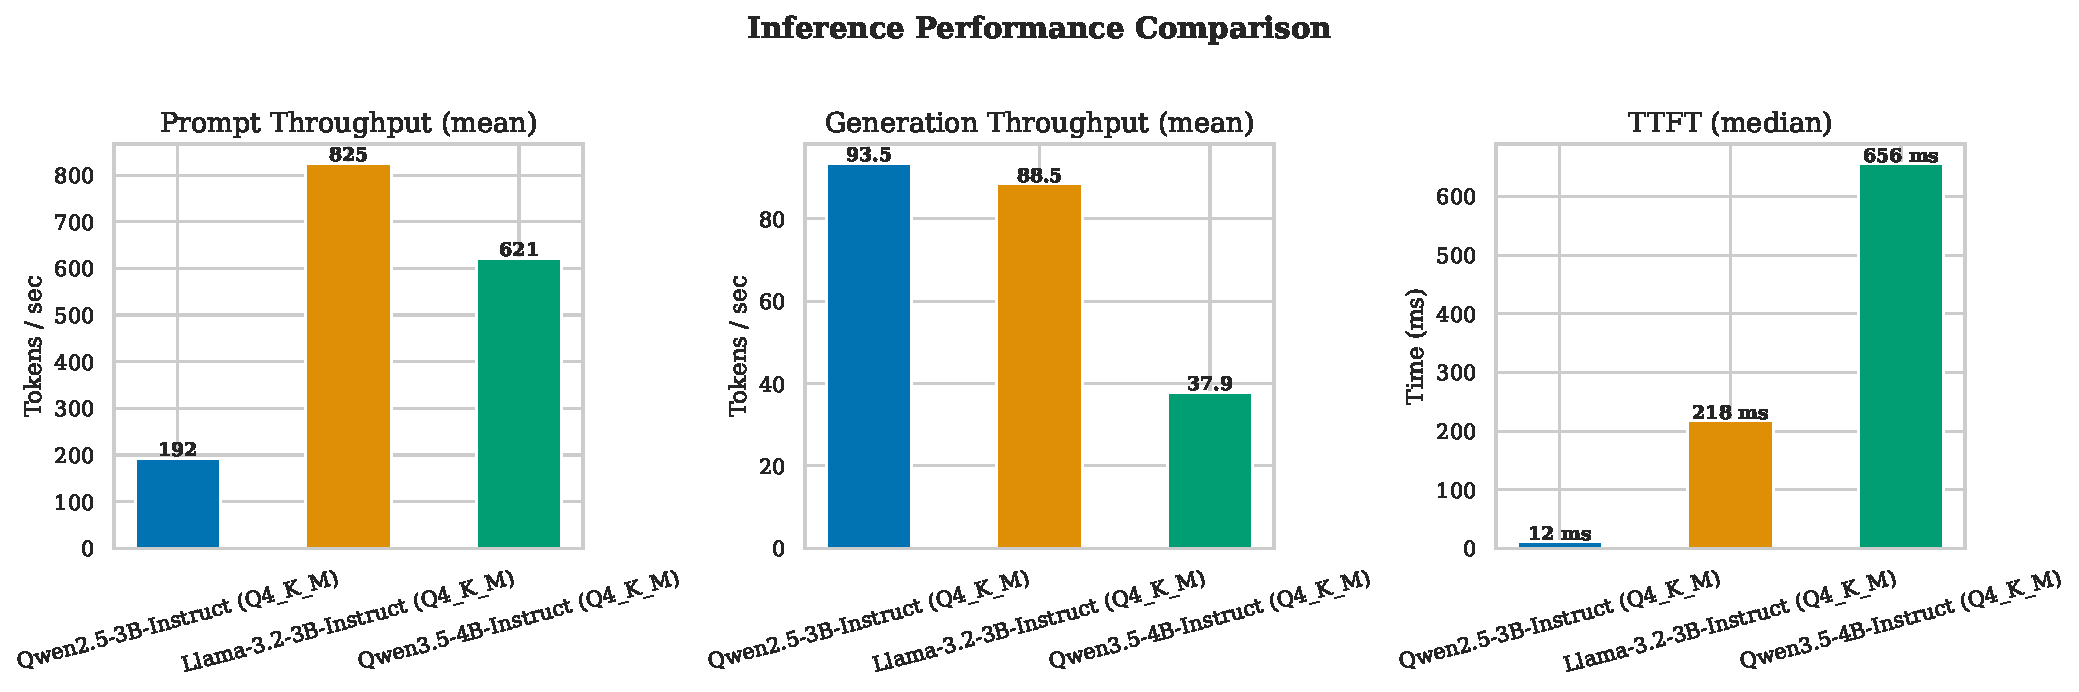
\includegraphics[width=0.92\textwidth]{performance_comparison.pdf}
\caption{Single-turn inference performance (prompt/generation throughput and time-to-first-token) for the four-model Mac comparison. Hardware: MacBook Pro M4~Pro, llama.cpp Metal. Fifty requests per model after warmup.}
\label{fig:perf}
\end{figure}

\begin{figure}[!htbp]
\centering
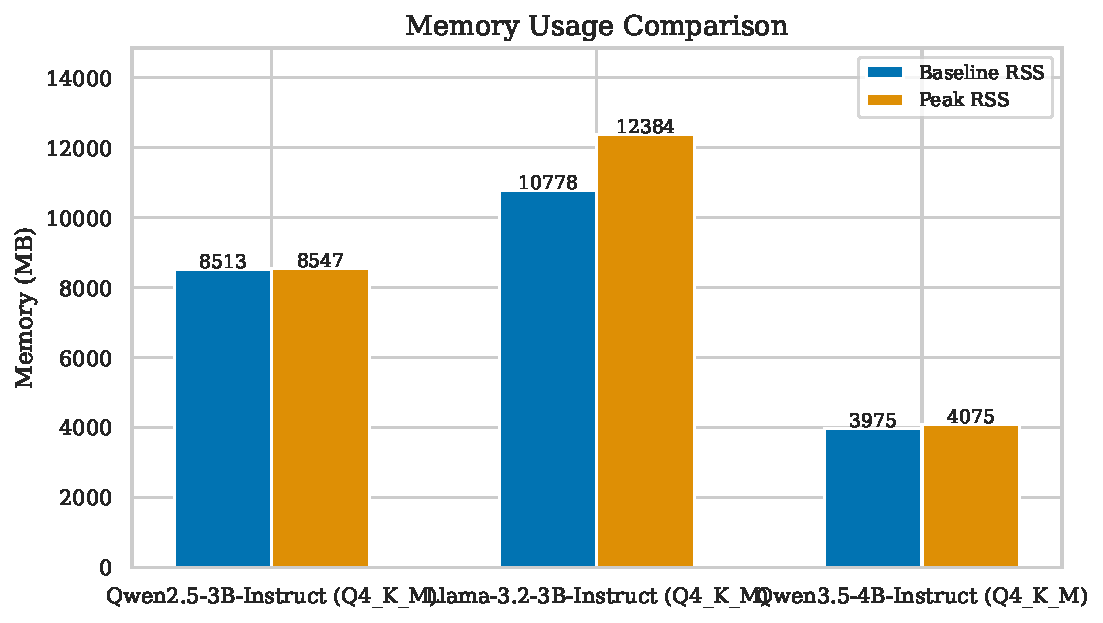
\includegraphics[width=0.92\textwidth]{memory_comparison.pdf}
\caption{Resident set size (RSS) baseline and peak during the same Mac M4~Pro / llama.cpp Metal metrics collection as Figure~\ref{fig:perf}.}
\label{fig:mem}
\end{figure}

\begin{table}[htbp]
\centering
\caption{Inference metrics on MacBook Pro M4~Pro / llama.cpp Metal (50 requests/model). Median generation throughput and median time-to-first-token (TTFT) are the headline latency numbers.}
\label{tab:perf}
\footnotesize
\begin{tabular}{@{}lrrrr@{}}
\toprule
Model & Gen.\ med.\ (tok/s) & TTFT med.\ (ms) & Peak RSS (MB) & Wtd.\ AST \\
\midrule
Qwen2.5-3B Q4\_K\_M & 93.6 & 11.6 & 8{,}546.9 & 76.06\% \\
Llama-3.2-3B Q4\_K\_M & 89.1 & 218.2 & 12{,}383.7 & 36.87\% \\
Qwen3.5-4B Q4\_K\_M & 38.0 & 656.3 & 4{,}075.4 & 82.53\% \\
FunctionGemma-270M bf16 & 204.2 & 16.2 & 6{,}562.2 & 39.90\% \\
\bottomrule
\end{tabular}
\end{table}

Mean prompt / generation throughput: Qwen2.5-3B 192.5 / 93.5 tok/s; Llama-3.2-3B 824.9 / 88.5 tok/s; Qwen3.5-4B 620.5 / 37.9 tok/s; FunctionGemma 2567.5 / 201.0 tok/s. Gemma NFC/CD/GST/STATE generation means (from stored inference metrics): 92.43 / 89.6 / 92.45 / 89.7 tok/s; peak RSS 15591 / 15531 / 15160 / 14867~MB. The IFFC baseline run has no inference-metrics row.

\FloatBarrier

\section{Discussion}
\label{sec:discussion}

\paragraph{Format versus reasoning.}
Several large swings are format. IFFC versus NFC, Llama type coercion, and xLAM's native-tools collapse all show that the channel the harness parses can dominate the score before agentic policy is tested. That is useful: format is often cheaper to fix than weights. It is also a warning. Publishing an overall BFCL number from a different channel, or treating NFC 0\% on xLAM as an ability floor, would mis-state the result.

Once calls parse, consecutive accuracy is limited by environment-state tracking. IFFC still shares 124 failures with NFC. STATE and BoN move the score by a few points and still leave VehicleControl and GorillaFileSystem mismatches as the mode. GST increases calling without reducing those mismatches. OODA-card raises accuracy while state-mismatch counts stay above the IFFC baseline. Constrained name decoding (CD, PTC-A) improves or enforces syntax and \emph{lowers} execution accuracy. Validity of a call is not fidelity of a trajectory.

\paragraph{Cost--accuracy.}
On base Gemma, the Pareto picture is: IFFC at 30.5\% as the cheap JSON channel; gated stop-repeat and OODA-card as low-overhead harness additions (32.5\% and 35.5\%); STATE at 34.0\% with extra context tokens; BoN at 36.5\% for about $7\times$ generate wall. For an edge agent, a 2.5\pp\ BoN gain at $7\times$ cost is a research measurement, not an obvious default. We did not apply BoN to collapsed or below-IFFC SFT checkpoints: majority vote cannot be assumed to rescue a policy that abstains or drifts.

\paragraph{Why SFT failed, then plateaued.}
The first SFT mixes taught the model to stop after tools because ToolACE empty-list targets dominate post-execution assistant turns. Removing those targets restores calling (empty errors $\approx 0$) but does not install BFCL-style state tracking. Further filters that try to complete turn~0 or drop state-inconsistent continues either over-call (v5) or miss the v4 recovery (v6). STATE, which helps the base model remember executed facts, is null or negative on the v4 checkpoint: the overlay is not a universal substitute for a policy that already mismatches the environment. Preference data that contrasts advance versus loop, rather than another supervised empty-list filter, is the remaining training hypothesis---untested at $N{=}200$ in this draft.

\paragraph{Paper IFFC versus the IFFC paper.}
Large lifts in~\cite{taheri2026iffc} are reported on single-turn Live/Non-Live suites, often where NFC is already weak, and often under dual QA / small-reasoner decoupling. Our Appendix~B-only multi-turn setup sits in a modest-gain band (${+}3.5$\pp). That is a different claim, not a refutation of theirs.

\section{Limitations and Roadmap}
\label{sec:roadmap}

Results are Apple Silicon / Metal only. Multi-turn coverage is Gemma-centric, plus an xLAM channel contrast. Parallel AST categories remain artifactual zeros. We do not invent scores for unfinished experiments, and we do not treat health-gate probes as BFCL percentages.

The following items are explicitly \emph{open}: no conclusion is claimed yet.

\begin{description}
  \item[DPO full train.] A $\beta{=}0.2$ 100-update smoke passed a 10-ID health gate. A capped full train is in flight. There is no $N{=}200$ DPO accuracy in this draft. Whether preference optimization beats IFFC 30.5\% or SFT-v4 15.0\% is unanswered.
  \item[Preference-pair audit.] Stage~B advance-versus-loop pairs are a draft engineering path, not a scored method.
  \item[Other models' multi-turn.] Qwen2.5-3B, Llama-3.2-3B, Qwen3.5-4B, and FunctionGemma-270M have single-turn numbers only.
  \item[Jetson Orin Nano Super.] CUDA / 8~GB replication of the Mac M4~Pro results is not run.
  \item[Dual-model IFFC.] Paper Algorithm~1 (QA LLM $+$ small reasoning model) is deferred; this draft uses Appendix~B JSON-in-text on one model.
  \item[Parallel categories.] Re-run after the llama-server tools GBNF truncation fix; tables still report 0\%.
  \item[OODA state mismatch.] The best non-BoN method still misses a clean state-mismatch reduction. Whether the card can be revised without losing the 35.5\% is open.
  \item[PTC-B.] Not pursued as the next accuracy bet. PTC-A is a scored failure; we do not remix prefix constraints next.
  \item[SFT after v4.] Quota remix is parked after the v9.2 smoke-gate fail. The next training story is preference/DPO, results pending---not more epochs on v5/v6 and not BoN on those checkpoints.
\end{description}

\section{Conclusion}
\label{sec:conclusion}

Quantized SLMs on a MacBook Pro M4~Pro with llama.cpp already achieve strong single-turn tool selection in the Qwen 3--4B family (weighted non-parallel AST up to 82.53\%), while FunctionGemma delivers interactive latency at 270M parameters. Much of Llama's \texttt{multiple} gap is serialization and is closable without weight updates.

For consecutive tool calling on Gemma-4-E2B-it, the story is narrower and more honest. Changing the output channel (IFFC) and adding cheap harness memory or guardrails moves \texttt{multi\_turn\_base} from 27.0\% into the low-to-mid 30s. Majority vote reaches 36.5\% at roughly $7\times$ cost. Constrained decoding and a live name automaton hurt. Supervised IFFC fine-tuning is easy to get spectacularly wrong (0.5\%) and, even after repairing empty-list targets, stalls at 15.0\%---below the untuned model. Residual failures are environment-state mismatches, especially on VehicleControl and filesystem backends, not unparsable JSON.

Preference optimization is the open training question: a DPO smoke is healthy, a full train is in flight, and this paper stops short of a BFCL conclusion. Completing that train, Jetson replication, other models' multi-turn baselines, dual-model IFFC, and parallel re-runs after the GBNF fix will determine how far local agents of this size can be pushed before December 2026.

\bibliographystyle{unsrtnat}
\bibliography{references}

\appendix
\section{Method caveats}
\label{app:caveats}

These distinctions are part of the method identity:

\begin{itemize}
  \item Constrained decoding is a two-pass TagDispatch-style approximation on stock llama-server, not full XGrammar-2.
  \item GST is a prompt overlay on NFC. It is not GBNF and not IFFC. The checker ignores GST drafts.
  \item STATE is a harness-written snapshot from executed tool results, not LLM summarization.
  \item Best-of-N is majority vote at $N{=}5$, not a learned verifier; generate wall is about $7\times$.
  \item Strip-empty (2.0\%) is serve-time history bookkeeping on the SFT-v2 GGUF, not a training method.
  \item SFT-v4 (15.0\%) is a recovery from 0.5\% collapse, not a win over IFFC or NFC.
  \item STATE on SFT-v4 (13.0\%) is a null/negative overlay: STATE helps base Gemma, not that checkpoint.
  \item xLAM 0\% / 3\% are this harness's native versus JSON channels, not published overall BFCL ${\sim}78.94\%$.
  \item PTC-A (13.5\%) is a closed accuracy failure, not Yu et al.'s reported F1.
  \item The DPO 10-ID result is a health-gate pass, not a BFCL percentage.
\end{itemize}

\section{Evaluation-log run IDs}
\label{app:runs}

Table~\ref{tab:runs} maps the method names used in the body to chronological IDs in the local SQLite evaluation log. IDs are bookkeeping; they are not needed to read the results.

\begin{table}[htbp]
\centering
\caption{Chronological evaluation-log IDs for scored \texttt{multi\_turn\_base} ($N{=}200$) rows, plus health gates that are not BFCL percentages. Gemma-4-E2B-it Q4\_K\_M unless noted.}
\label{tab:runs}
\footnotesize
\begin{tabular}{@{}rllr@{}}
\toprule
ID & Method name in this paper & Acc. & Role \\
\midrule
4 & NFC & 27.0\% & native baseline \\
5 & IFFC & 30.5\% & JSON-in-text baseline \\
8 & Constrained decoding & 10.5\% & scored negative \\
9 & GST$+$NFC & 30.5\% & tie with IFFC \\
10 & IFFC$+$STATE & 34.0\% & harness memory \\
11 & Best-of-N $N{=}5$ & 36.5\% & best inference \\
12 & SFT-v1 & 0.5\% & empty-\texttt{[]} collapse \\
13 & SFT-v2 & 0.5\% & filter did not recover \\
14 & Strip trailing \texttt{[]} & 2.0\% & diagnostic \\
15 & SFT-v4 & 15.0\% & best SFT recovery \\
16 & SFT-v4 $+$ STATE & 13.0\% & null/negative overlay \\
17 & SFT-v5 & 11.5\% & regression vs v4 \\
18 & SFT-v6 & 13.0\% & miss vs v4 \\
19 & xLAM-1b NFC & 0.0\% & format collapse \\
20 & xLAM-1b JSON channel & 3.0\% & fair channel, still low \\
27 & Ungated stop-repeat & 27.0\% & miss vs IFFC \\
30 & Gated stop-repeat & 32.5\% & ${+}2.0$\pp vs IFFC \\
36 & SFT v9.2 smoke (10 IDs) & --- & health-gate FAIL; not BFCL \% \\
42 & OODA-card & 35.5\% & best non-BoN \\
46 & PTC-A & 13.5\% & scored failure; line closed \\
49 & DPO $\beta0.2$ smoke (10 IDs) & --- & health-gate PASS; not BFCL \% \\
\bottomrule
\end{tabular}
\end{table}

\section{Acronyms}
\label{app:acro}

\begin{table}[htbp]
\centering
\caption{Acronyms used in the paper.}
\label{tab:acro}
\small
\begin{tabular}{@{}lp{11.4cm}@{}}
\toprule
Acronym & Meaning \\
\midrule
AST & Abstract syntax tree checker (single-turn BFCL scoring) \\
BFCL & Berkeley Function Calling Leaderboard \\
BoN & Best-of-N; here, majority vote over sampled tool-call tuples \\
CD & Constrained decoding (our two-pass TagDispatch-style ablation) \\
DPO & Direct Preference Optimization \\
GBNF & GGML Backus--Naur Form grammar used by llama.cpp \\
GST & Guided-structured templates (He et al.; prompt overlay here) \\
IFFC & Instruction-followed function calling (JSON-in-text) \\
NFC & Native function calling (OpenAI-style \texttt{tool\_calls}) \\
OODA & Observe--orient--decide--act; here, a one-pass status card \\
PTC-A & Prefix-tree / DFA constraint on tool names, arguments free \\
SFT & Supervised fine-tuning \\
SLM & Small language model ($<5$B parameters in this paper) \\
STATE & Harness-written working-memory snapshot from executed tools \\
TTFT & Time to first token \\
\bottomrule
\end{tabular}
\end{table}

\end{document}
